\chapter{场景建模与测试生成方法}
    \section{场景模型定义}
        \textbf{使用场景模型}是一种有效的模型化技术. 使用场景模型可以描述在现实世界中, 一或多个人如何与系统进行交互\footnote{http://agilemodeling.com/artifacts/usageScenario.htm}. 模型表达了交互过程中的步骤, 事件和动作. 本文提出了一种描述与web API交互的使用场景模型. 为了基于模型进行测试生成, 模型着重于抽象以下web API的特点:
        
        \begin{itemize}
            \item 与使用场景相关的服务元素. 这包括服务的功能, 请求数据, 响应数据, 执行约束等.
            
            \item 交互中各服务之间的交互与通信. 这包括执行序列和序列内消息传递, 比如调用序列中之前某个服务的响应, 可能作为之后调用其他服务的参数.
            
            \item 不同交互操作的频率. 在有限测试资源的情况下, 对于测试资源的分配, 各个被测API需要有优先级顺序. 比如, 一些API可能在许多场景下都被频繁调用, 或者为许多其他API提供前置服务. 那么, 根据基于使用的测试原则, 这些频繁使用的API需要进行更多测试. 因此, 对API使用的分析与建模有助于优化对各个API生成的测试用例数量.
        \end{itemize}
        
        概率有限状态自动机(PFSA)可以有效描述相关服务, 执行序列和交互频率. 然而, 对于数据约束和服务间消息传递, 它的能力有所不足. 我们的模型基于概率有限状态自动机进行扩展, 克服了这些不足.
        
        \subsection{背景: 概率有限状态自动机}
        
            概率有限状态自动机(PFSA)是非确定性有限状态自动机(NFA)的扩展. 它将概率因素引入非确定性有限状态自动机的转移, 起始状态和终止状态中. 对于每个串中读入的字符, 自动机会根据从当前状态出发的转移边的概率分布, 来从可选的一或多条转移边中选择一项进行转移. 状态的初始和终止也具有类似的概率性质.
            
            根据Enrique Vidal等人的阐述\cite{enriquev05}, 一个基本的概率有限状态自动机具有如下的定义(定义\ref{def.pfsa}).
            
            \begin{definition}
                \label{def.pfsa}
                概率有限状态自动机为一个元组
                \begin{equation}
                    \mathcal{B} := <Q_{\mathcal{B}}, \Sigma, \sigma_{\mathcal{B}}, I_{\mathcal{B}}, F_{\mathcal{B}}, P_{\mathcal{B}}>,
                \end{equation}
                
                其中:
                \begin{itemize}
                    \item $Q_{\mathcal{B}}$是有限的状态集合;
                    
                    \item $\Sigma$是字符集;
                    
                    \item $\sigma_{\mathcal{B}} \subseteq Q_{\mathcal{B}} \times \Sigma \times Q_{\mathcal{B}}$是状态转移的集合;
                    
                    \item $I_{\mathcal{B}} : Q_{\mathcal{B}} \to \mathbb{R}^{+}$是各个状态作为起始状态的概率分布;
                    
                    \item $F_{\mathcal{B}}: Q_{\mathcal{B}} \to \mathbb{R}^{+}$是于各个状态处终止的概率分布;
                    
                    \item $P_{\mathcal{B}} : \sigma_{\mathcal{B}} \to \mathbb{R}^{+}$是各条转移边的转移概率.
                \end{itemize}
                
                $I_{\mathcal{B}}$函数满足初始状态概率归一化性质:
                \begin{equation}
                    \sum_{q \in Q_{\mathcal{B}}} I_{\mathcal{B}}(q) = 1.
                \end{equation}
                
                $F_{\mathcal{B}}$和$P_{\mathcal{B}}$函数满足转移概率归一化性质:
                \begin{equation}
                    \forall q \in Q_{\mathcal{B}}, \forall a \in \Sigma, F_{\mathcal{B}}(q) + \sum_{q' \in Q_{\mathcal{B}}} P_{\mathcal{B}}(q,a,q') = 1.
                \end{equation}
            \end{definition}
            
            按照惯例, 概率有限状态自动机使用带标签边的有向图表示. 图\ref{fig:PFSA_example}展示了一个概率有限状态自动机的例子. 其中, 图的节点表示自动机的状态, 图的带标签边表示自动机的概率转移边, 图中节点上的数字表示自动机状态的终止概率.
            
            \begin{figure}[!htb]
                \centering
                
\includegraphics[width=300pt]{PFSA_example.pdf}
                \caption{概率有限状态自动机的可视化表示}
                \label{fig:PFSA_example}
            \end{figure}
            
            概率有限状态自动机是一种随机模型, 它生成的是在有限串集合$\Sigma^{*}$上的概率空间. 对于此自动机, 生成一个串的步骤为:
            
            \begin{itemize}
                \item 初始化: 按照概率分布$I_\mathcal{B}$选择一个$Q_{\mathcal{B}}$中的状态$q_0$作为初始状态;
                
                \item 生成: $q$表示当前状态, $a$表示当前读入字符. 则以$F_{\mathcal{B}}(q)$的概率决定是否在此状态处终止, 或者以$P_{\mathcal{B}}(q, a, q')$的概率决定是否进行转移$(q,a,q')$. 如果进行此转移, 则将$q'$置为当前状态.
            \end{itemize}
        
            概率有限状态自动机的以下特点让其适用于使用场景的建模:
            
            \begin{itemize}
                \item 自动机的状态可以很方便地与服务端点关联起来. 因此, 状态序列可建模服务端点的调用与执行序列.
                
                \item 自动机的字符集$\Sigma$可建模服务端点的所有可能的响应. 另一方面, 每个状态转移均对应一个字符$c \in \Sigma$, 其表示此转移仅限当前读入字符为$c$时使用. 因此, 此字符可建模各个转移所适用的范围, 此范围由服务端点的返回响应决定. 也就是状态转移对应的字符定义了进行此状态转移的条件.
                
                \item 自动机的起始概率, 终止概率, 转移概率反映了与各服务端点进行交互的频率差异.
            \end{itemize}
            
            然而, 在使用场景模型中关键的数据流信息, 如数据约束, 数据依赖, 测试断言等, 则很难在概率有限状态自动机中表达与反映. 本文的场景模型扩展了概率有限状态自动机模型来克服这一问题.
        
        \subsection{形式化定义}
            本文的场景模型在以下两方面扩展了基本的概率有限状态自动机:
            
            \begin{itemize}
                \item 它在状态定义中加入了请求数据约束与请求数据依赖的定义, 以便于生成请求数据.
                
                \item 它在状态定义中加入了响应数据约束与测试断言 的定义, 以便于对响应进行验证.
            \end{itemize}
            
            形式化的定义如下:
            
            \begin{definition}
                \label{def:our}
                场景模型是一个元组
                \begin{equation}
                     \mathcal{A} := <Q_{\mathcal{A}}, \Sigma, \sigma_{\mathcal{A}}, I_{\mathcal{A}}, F_{\mathcal{A}}, P_{\mathcal{A}}>,
                \end{equation}
                
                其中:
                \begin{itemize}
                    \item $Q_{\mathcal{A}}$是有限的状态集合;
                    
                    \item $\Sigma$是所有可能的API响应的集合;
                    
                    \item $\sigma_{\mathcal{A}} \subseteq Q_{\mathcal{A}} \times \Sigma \times Q_{\mathcal{A}}$是状态转移的集合;
                    
                    \item $I_{\mathcal{A}} : Q_{\mathcal{A}} \to \mathbb{R}^{+}$是各个状态作为起始状态的概率分布;
                    
                    \item $F_{\mathcal{A}} : Q_{\mathcal{A}} \to \mathbb{R}^{+}$是于各个状态处终止的概率分布;
                    
                    \item $P_{\mathcal{A}}: \sigma_{\mathcal{A}} \to \mathbb{R}^{+}$是各条转移边的转移概率.
                \end{itemize}
                
                对于$I_{\mathcal{A}}$, $F_{\mathcal{A}}$, $P_{\mathcal{A}}$, 仍然要求满足归一化性质:
                \begin{equation}
                    \sum_{q \in Q_{\mathcal{A}}} I_{\mathcal{A}}(q) = 1;
                \end{equation}
                与
                \begin{equation}
                    \forall q \in Q_{\mathcal{A}}, \forall a \in \Sigma, F_{\mathcal{A}}(q) + \sum_{q' \in Q_{\mathcal{A}}} P_{\mathcal{A}}(q,a,q') = 1.
                \end{equation}
                
                状态$q \in Q_{\mathcal{A}}$的定义是一个元组
                \begin{equation}
                    q := <t_q, in_q, out_q, d_q, a_q>,
                \end{equation}
                其中:
                \begin{itemize}
                    \item $t_q$可以为$empty$(表示不与任何API服务端点关联)或某个服务端点的名称;
                    
                    \item $in_q$是当前状态所有合法请求数据的集合;
                    
                    \item $out_q$是当前状态所有合法响应体的集合;
                    
                    \item $d_q$是请求数据依赖的集合;
                    
                    \item $a_q$是响应体断言的集合.
                \end{itemize}
                
                作为所有可能的API响应的集合, $\Sigma$满足
                \begin{equation}
                    \Sigma = \bigcup_{q \in Q_{\mathcal{A}}} out_q.
                \end{equation}
                
                在状态$q$的定义中, 每一项请求数据依赖$d \in d_q$都是一个元组
                \begin{equation}
                    d := <q_d, index_d, f_d>,
                \end{equation}
                它的各项含义为:
                \begin{itemize}
                    \item $q_d \subseteq Q_{\mathcal{A}}$是场景模型$\mathcal{A}$中的一个或多个状态的集合;
                    
                    \item $index_d \in \mathbb{Z}$是一个整数;
                    
                    \item $f_d: \bigcup_{q' \in q_d} in_{q'} \times out_{q'} \to i \subseteq in_q$是一个函数, 此函数定义了给定状态$q_d$上的请求数据和得到的响应, 对当前状态$q$而言, 合法的请求数据集合.
                \end{itemize}
                
                在状态$q$的定义中, 每一项响应体的断言$a \in a_q$也是一个元组
                \begin{equation}
                    a := <q_a, index_a, f_a>,
                \end{equation}
                它的各项含义为:
                \begin{itemize}
                    \item $q_a \subseteq Q_{\mathcal{A}}$是场景模型$\mathcal{A}$中的一个或多个状态的集合;
                    
                    \item $index_a \in \mathbb{Z}$是一个整数;
                    
                    \item $f_a: \bigcup_{q' \in q_a} in_{q'} \times out_{q'} \to o \subseteq out_q$是一个函数, 此函数定义了给定状态$q_a$上的请求数据和得到的响应, 对当前状态$q$而言, 合法的响应数据集合.
                \end{itemize}
            \end{definition}
            
            需要注意的是, 在web API测试的语义下, 输入数据是测试方法所生成的, 也就是对某个API服务端点的请求数据. 输出数据则是API返回的响应体, 有时也包括响应头的某些域.
        
        \subsection{解释与说明}
            在本文的场景模型中, 对输入数据的约束集合$in_q$附在每个状态$q$上. 输入数据的约束集合定义了输入数据的取值空间, 即满足约束的数据构成了输入数据的取值空间, 数据的生成就是为此取值空间赋予概率分布, 然后进行随机采样. 对输出数据的约束集合$out_q$也附在每个状态$q$上, 使用输入数据请求对应API服务端点, 得到的响应使用约束条件进行验证, 便可以检验API的行为是否符合定义.
            
            输入数据的依赖$d := <q_d, index_d, f_d >$则表达了由上下文对当前状态的请求数据赋予的额外约束. 其具体含义为: 在模型上遍历的同时记录下当前的状态序列, 然后保序提取出属于$q_d$的状态, 找出其中的第$index_d$项状态(下标$index_d$从0开始, 负数表示倒数第$|index_d|$项状态). 此时, $(q_d, index_d)$指向了当前状态序列中某一个确定状态元素$now$. 然后, 提取出该状态执行时的请求数据(即输入, 记为$i_{now}$)与响应(即输出, 记为$o_{now}$), 再应用到函数$f_d$, 得到的$f_d(i_{now}, o_{now})$定义了当前状态(更严格的)合法请求数据(即输入数据)集合. 可以看出, 合法输入数据的集合由当前执行状态序列中之前的输入输出决定.
            
            响应体的断言$a := <q_a, index_a, f_a>$的具体含义也相似. 这里, $f_a(i_{now}, o_{now})$定义的是当前状态(更严格的)合法响应(即输出数据)集合.
            
            $f_d$和$f_a$函数虽然取上下文中之前的输入和输出数据作为参数, 但也可以不依赖于这两项, 此时, 则相当于直接对当前状态施加额外的输入数据限制和输出断言, 作用与$in_q$和$out_q$相似. 不过, 在具体实现时, $in_q$和$out_q$是由API行为描述文档引入的, 而$f_d$和$f_a$定义在场景模型描述脚本内.
        
        \subsection{示例}
            \begin{figure}[!htb]
                \centering
                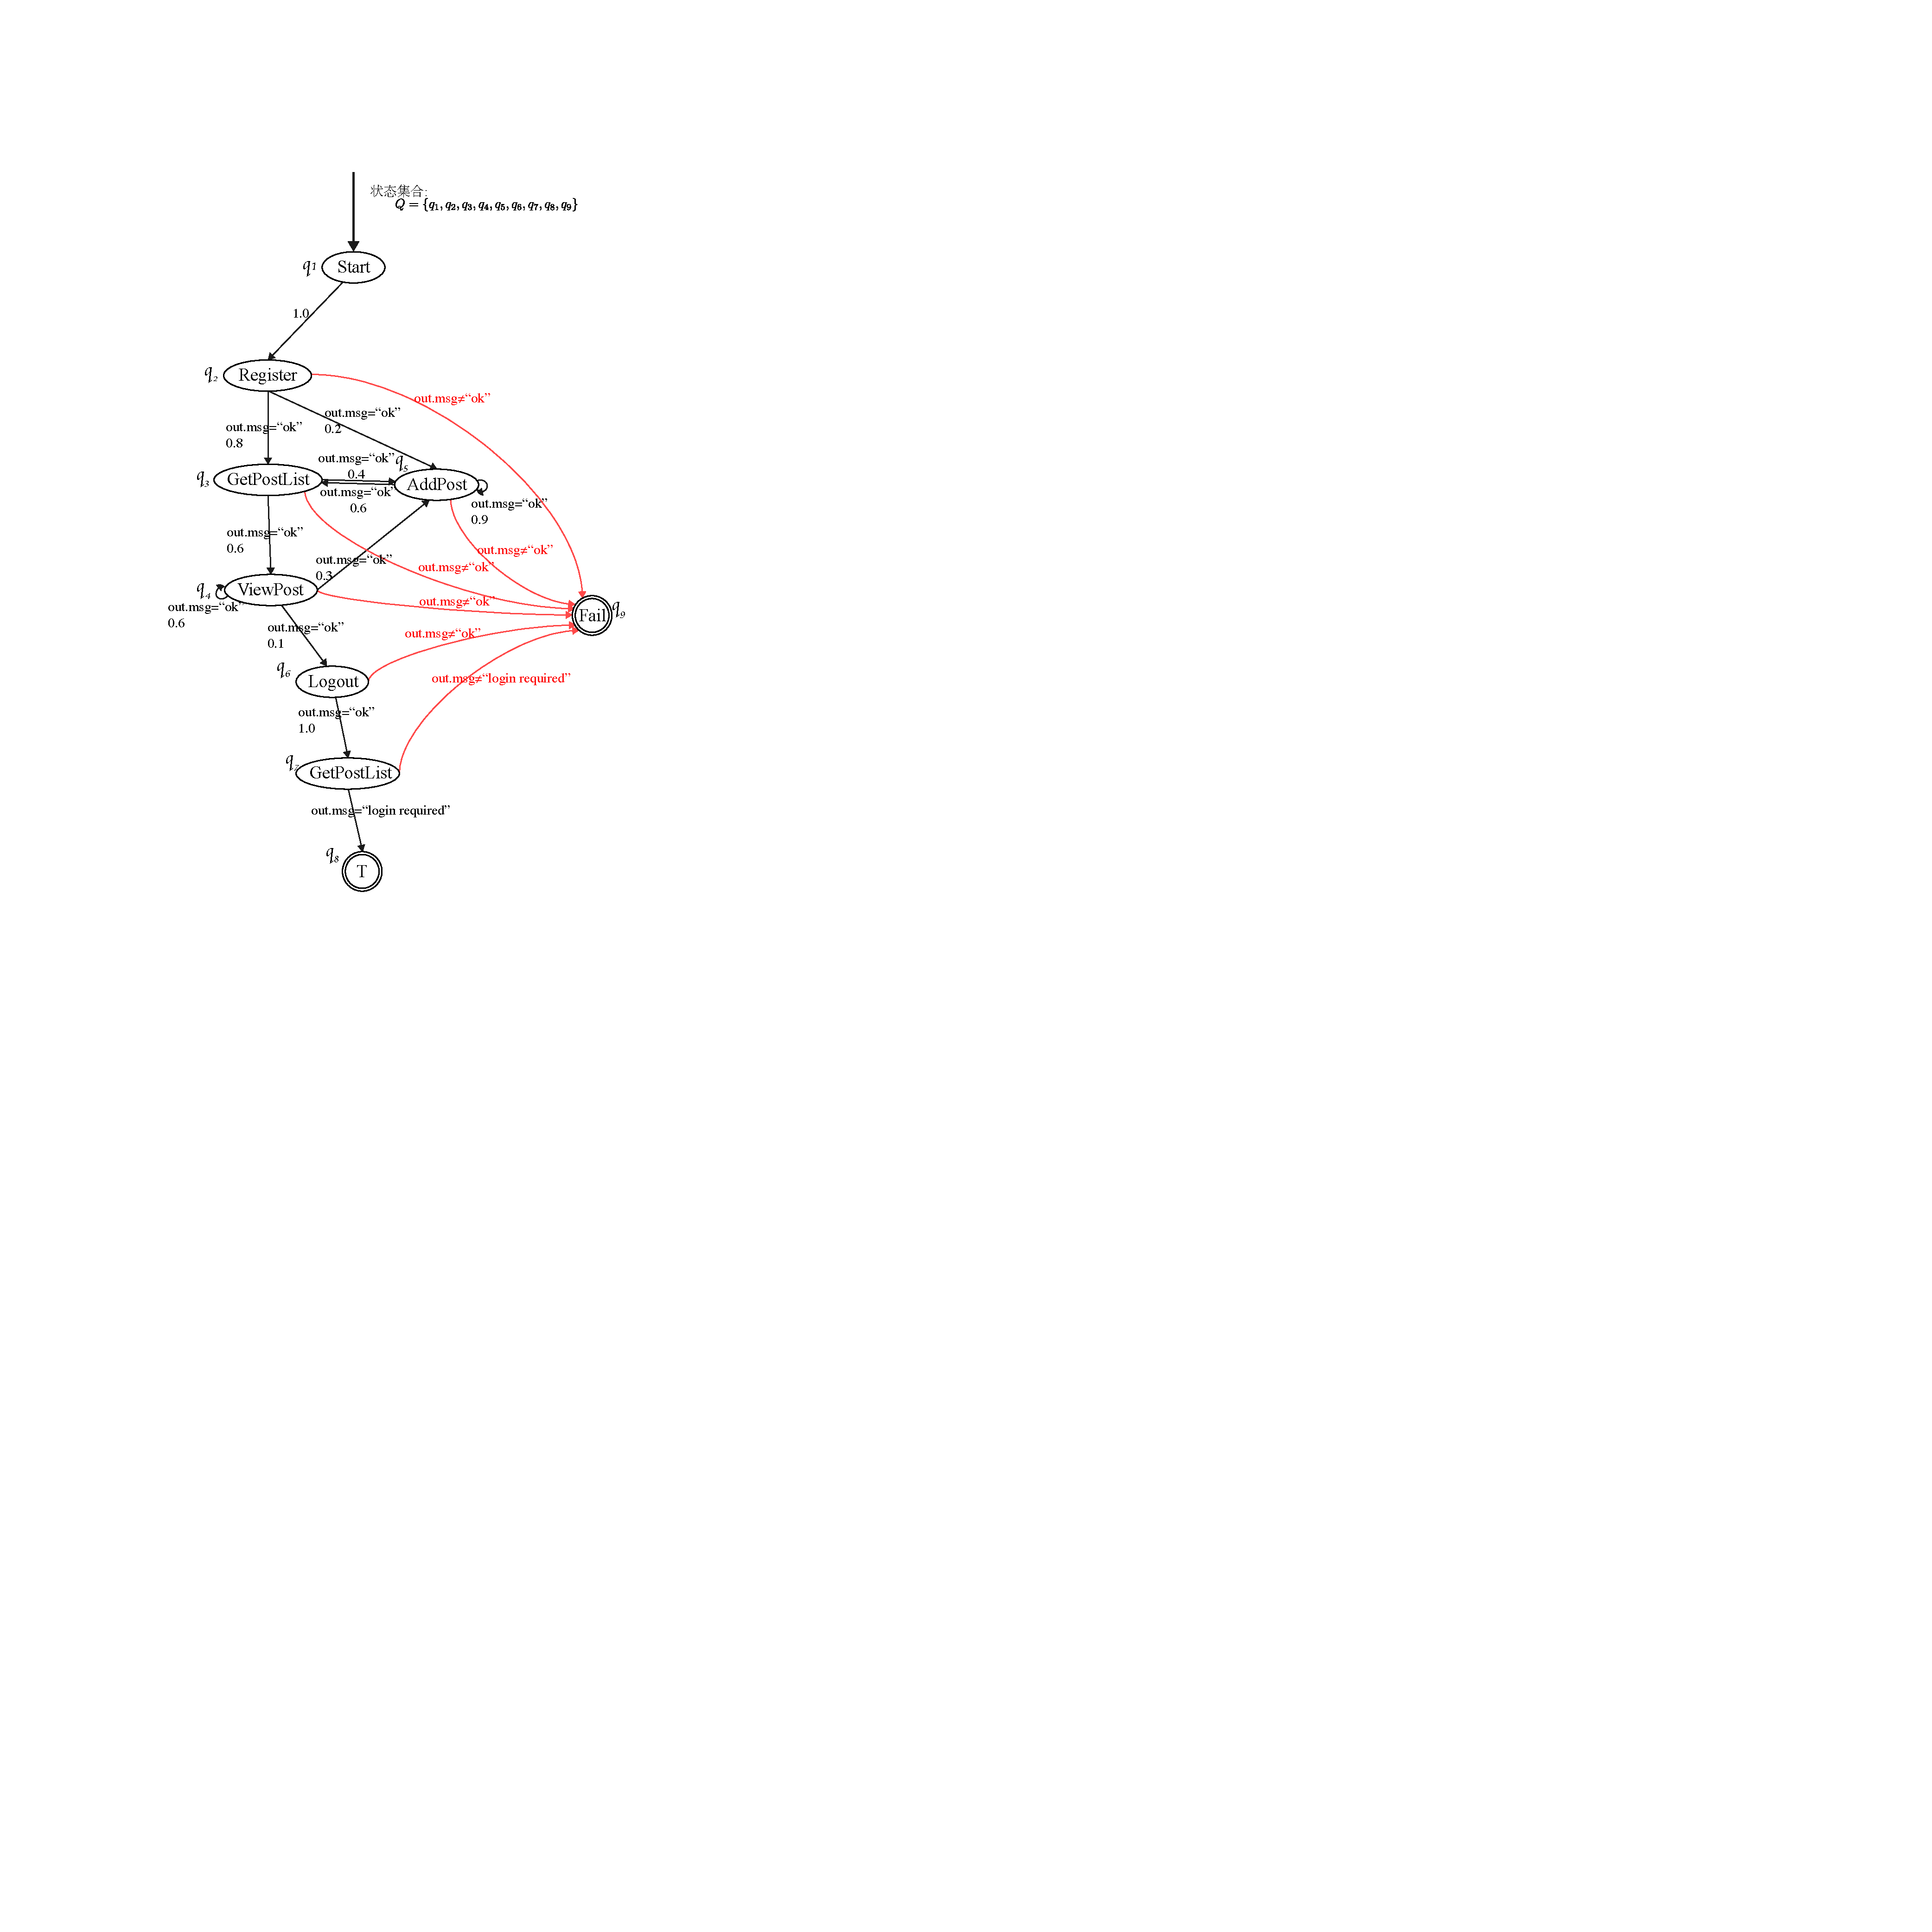
\includegraphics[width=300pt]{scenario_example.pdf}
                \caption{一个场景模型的实例. 输入数据依赖和响应体断言为: \\
                $q_3$.\texttt{request.username} = $q_2$.\texttt{request.username};\\
                $q_3$.\texttt{request.ssid} = $q_2$.\texttt{response.ssid};\\
                $q_4$.\texttt{request.username} = $q_2$.\texttt{request.username};\\
                $q_4$.\texttt{request.postId} = $q_3$.\texttt{response.posts}.\\
                这里, 状态集合的定义($q_d$, $q_a$)和函数的定义($f_d$, $f_a$)以以上谓词形式给出. 起始状态为$q_1$, 终止状态为$q_8, q_9$, 是确定性的.}
                \label{fig:scenario_example}
            \end{figure}
            
            图\ref{fig:scenario_example}为一个典型的场景模型的示例. 这个场景模型是为一个类似微博的自媒体平台服务设计的. 在这个服务里, 用户可以登录, 浏览微博, 发布新微博. 服务开发的5个API接口为: “Register”(注册)、“GetPostList”(获取动态)、“ViewPost”(浏览微博)、“AddPost”(发布)、“Logout”(登出). 在图中, 类似自动机的表示方法, 使用图的节点来表示场景模型的状态, 使用图的边表示场景模型的转移, 边上的数字表示转移概率, 边上的文字表示转移条件. 示例中共有9个状态和18项转移. 初始状态只有一个, 为$q_1$(“Start”). 终止状态有两个, 为$q_8$和$q_9$(“T”和“Fail”). 这里的初始状态和终止状态是确定性的($I(\cdot) \in {0,1}$, $F(\cdot) \in {0,1}$), 但模型本身也支持概率性的. 除了初始状态和终止状态, 示例中其他的状态均与API服务端点关联, 图中对应节点上的标签即为关联API的名称. 处于这些状态时, 就会向这些对应API发送请求. 举例来说, $q_2$对应注册API, $q_3$对应获取动态的API. 在转移边上, 标出的转移概率可以反映出实际使用场景下, 不同执行路径的频率.
        
        \subsection{构建与实现}
            场景模型抽象了API的使用场景, 并为生成高效的测试用例提供了必需的知识. 目前, 场景模型需要手工进行构建与设计, 然后才能自动生成与执行测试用例. 未来, 将进一步探索如何从自然语言描述和日志文件中进行自动化场景生成
            
            场景模型使用与OpenAPI规约语言类似的规约语言描述, 并用YAML格式记录.
            
            在具体实现上, 合法输入(包括输入依赖), 合法响应(包括输出断言), 转移条件的定义($in_q$, $out_q$, $f_d$, $f_a$, $x \in Sigma$)的定义有多种来源:
            
            \label{sec:set_define}
            \begin{itemize}
                \item JSON模式(JSON Schema)\footnote{https://tools.ietf.org/html/draft-wright-json-schema-validation-00}.\\
                JSON模式被用于结构化JSON数据的验证. 对于一个JSON模式定义而言, 通过验证的数据构成了一个固定集合. 当所需集合不依赖于其他状态(即上下文)时, 便可以使用JSON模式定义. 在使用OpenAPI描述的API脚本文档中, 均采用这种方法定义合法输入和合法响应. 场景模型中的状态定义如果关联了一个API服务端点, 则默认将此API的脚本文档中的合法输入, 合法响应的定义作为该状态的合法输入, 合法响应定义. 此外, 由于输入依赖和输出断言需要定义依赖上下文的函数($f_d$, $f_a$), 一般不使用JSON模式定义. 
                
                \item 自定义校验函数.\\
                本文的工具原型支持可扩展插件. 用户可以编写并引入校验函数, 校验函数接受数据作为输入, 判定数据是否满足条件. 因此, 满足条件的数据构成了一个集合. 这种定义方式只能在合法响应(包括输出断言)和转移条件的定义中使用, 而不能用于定义合法输入, 因为定义合法输入时还需要在定义的集合中采样, 而只判定是否属于某集合的函数显然不具备此功能.
                
                \item 自定义生成函数.\\
                用户可以编写并引入生成函数, 生成函数要求随机返回一个在其隐式定义的集合内的元素. 生成函数可以用于定义合法输入(包括输入依赖), 这是因为测试时只需要获得满足条件的数据即可. 但是, 由于生成函数不能判定某个数据是否属于其定义的集合, 也不能获取其定义集合的所有元素. 所以它不能用于定义合法响应和转移条件.
            \end{itemize}
            
    
    \section{测试生成方法}
        现在, 有了OpenAPI规约语言描述的API行为文档, 和场景模型, 接下来的任务就是生成并执行测试了. 测试的生成有两个层次: 一个是为单次API请求生成请求数据(即输入数据), 一个是将单个请求串联起来生成API执行序列作为测试用例.
        
        \subsection{请求数据生成}
            请求数据的生成, 就是在合法请求数据集合中的随机采样. \ref{sec:set_define}小节总结了目前支持的集合定义方法: 在定义合法输入时, 有JSON模式和自定义生成函数两种定义方法.
            
            当合法输入使用JSON模式定义时, 由于每个数据结构都属于JSON模式定义的基本类型之一, 因此, 分类讨论为每个基本类型设计采样策略即可. 此外, 对于一些特殊子类型如日期、时间、二进制串等, 本文定义了特殊采样策略. 具体策略见表\ref{tab:schemagen}. 特别地, 当多个条件均满足时, 则合理结合多个策略生成.
            
            \begin{table}[!htb]
                \centering
                \begin{tabular}{rll}
                    \toprule
                    类型 & 条件 & 策略 \\
                    \midrule
                    null & / & 返回元素\texttt{Null} \\
                    \hline
                    integer \& & 存在\texttt{multipleOf}域 & 从满足倍数关系的值空间中采样 \\
                    \cline{2-3}
                    float & 存在\texttt{enum}域 & 从定义的有限集合中采样 \\
                    \cline{2-3}
                    & 存在\texttt{MIN}或\texttt{MAX}域 & 从定义的区间中采样 \\
                    \cline{2-3}
                    & / & 在对应类型的整个区间中采样 \\
                    \hline
                    boolean & 存在\texttt{enum}域 & 从定义的有限集合中采样 \\
                    \cline{2-3}
                    & / & 使用伯努利分布($p=0.5$) \\
                    \hline
                    string & 存在\texttt{regex}域 & 从正则表达式定义的模式中生成 \\
                    \cline{2-3}
                    & 存在\texttt{enum}域 & 从定义的有限集合中采样 \\
                    \cline{2-3}
                    & \texttt{format}域存在 & 先随机日期, \\
                    & 且为\texttt{'date'} & 再以RFC3339的full-date格式表示 \\
                    \cline{2-3}
                    & \texttt{format}域存在 & 先随机日期时间, \\
                    & 且为\texttt{'datetime'} & 再以RFC3339的date-time格式表示 \\
                    \cline{2-3}
                    & \texttt{format}域存在 & \multirow{2}{*}{随机二进制串, 以\texttt{bytes}格式返回} \\
                    & 且为\texttt{'binary'} &  \\
                    \cline{2-3}
                    & 存在\texttt{minLength} & 先从指定长度区间随机长度值, \\
                    & 或\texttt{maxLength}域 & 再随机生成字符串 \\
                    \cline{2-3}
                    & \multirow{2}{*}{/} & 先随机确定长度值(默认不超过255),\\
                    & & 再随机生成字符串 \\
                    \hline
                    array & 存在\texttt{maxItems} & 先从指定区间随机列表长度,\\
                    & 或\texttt{minItems}域 & 再随机递归生成各元素 \\
                    \cline{2-3}
                    & \multirow{2}{*}{/} & 先随机确定列表长度,\\
                    & & 再随机递归生成各元素 \\
                    \hline
                    object & / & 递归生成各成员 \\
                    \bottomrule
                \end{tabular}
                \caption{从JSON模式生成请求数据. 依据基本类型和条件分类讨论, 采取不同策略.}
                \label{tab:schemagen}
            \end{table}
            
            当合法输入使用自定义生成函数定义时, 由于函数期望的返回值就是其隐式定义的集合的采样, 故直接将返回值作为请求数据即可.
        
        \subsection{执行序列生成}
            如果以自动机的视角审视场景模型, 那么它所定义的仍然是合法串的集合以及它们的概率分布. 由于每个自动机的状态可以与一个API服务端点关联, 所以产生的串也可以对应于API的请求/执行序列. 在进行web API测试时, 一个这样的包含具体请求数据的序列, 即是一个测试用例.
            
            因此, 执行序列生成算法的基本思想, 就是根据场景模型定义的概率分布生成可以被其接受的串. 相比看似相近的概率图模型和马尔科夫模型, 场景模型中转移到某一状态不仅仅由当前状态和概率分布决定. 由于每项转移是否可用取决于关联的API服务端点的响应结果, 而API服务端点的响应结果取决于输入的请求数据, 请求数据的生成过程依赖整个当前序列, 故状态转移还可以与之前的所有状态均相关. 因此, 场景模型的表达能力要强于仅与当前状态和概率分布相关的概率图模型与马尔科夫模型.
            
            执行序列生成算法的大体流程如算法\ref{algo:seqgen}所示.
            
            在算法\ref{algo:seqgen}中, 首先, 根据初始状态概率分布函数$I_{\mathcal{A}}$随机选择初始状态. \texttt{RandomChoice()}函数接受两个列表作为参数, 分别表示候选元素和每个元素的概率权重, 它按照权重随机抽取一个元素作为返回值, 故\texttt{RandomChoice(}$Q_{\mathcal{A}}$\texttt{,}$I_{\mathcal{A}}$\texttt{)}返回随机选择的初始状态. 然后, 算法在自动机上进行遍历. 每一步中, 使用$current$记录当前所处状态, 请求数据和响应数据等上下文信息. $r$是存储整个序列的上下文信息的总列表. 如果当前状态与一个API服务端点相关联, 算法将遍历请求数据的各个参数定义, 并从数据依赖定义或合法集合定义中随机生成出参数. 之后, 算法发送请求并解析响应体. 解析完成后, 算法扫描响应的各个域, 根据断言定义或合法集合定义进行验证, 如果验证不通过, 算法终止. 最后, 算法根据终止概率分布函数$F_{\mathcal{A}}$进行概率终止, 若未终止, 则根据响应和转移概率函数$P_{\mathcal{A}}$随机选择下一状态, 进入下一步.
            
            当算法结束时, 返回的值包括执行序列$r$和终止原因$T$, 其中终止原因$T$详细记录了跳出算法循环的位置和具体信息, 便于发现被测系统故障时进行修复.
            
            从描述中可以看出, 算法结合了执行序列的生成和执行过程, 并且生成过程实时受执行结果(即API响应)的反馈影响. 序列生成是动态的, 这使预处理相关的加速和优化变得困难, 但也使生成的序列更为灵活, 更为贴近实际使用场景.
            
            \begin{algorithm}
              	\scriptsize
              	
                \caption{API执行序列生成算法}
              	
                \KwIn{$Spec$, $\mathcal{A}$} 
                \tcp{输入: API定义脚本和场景模型脚本}
                \tcp{场景模型$\mathcal{A} := <Q_{\mathcal{A}}, \Sigma, \sigma_{\mathcal{A}}, I_{\mathcal{A}}, F_{\mathcal{A}}, P_{\mathcal{A}}>$}
                \KwOut{$r$, $T$}
                \tcp{输出: 执行序列和终止原因}
                $q$ $\gets$ RandomChoice($Q_{\mathcal{A}}$, $I_{\mathcal{A}}$)\;
                \tcp{根据初始状态概率分布函数随机初始状态$q := <t_q, in_q, out_q, d_q, a_q>$}
                $current$ $\gets$ $EmptyMap$\;
                $current.state$ $\gets$ $q$\;
                $r$ $\gets$ $EmptyList$\;
                $stop$ $\gets$ $false$\;
                \While {$\neg stop$} {
                	$i$ $\gets$ $EmptyMap$\;
                    $o$ $\gets$ $EmptyMap$\;
                	\If(\tcp*[h]{$q$有关联的API服务端点}) {$t_q \neq empty$}{
                    	\ForEach(\tcp*[h]{遍历处理所有请求参数}) {$param$ in $t_q.params$} {
                        	\If(\tcp*[h]{当前参数$param$有数据依赖, 则从依赖生成请求数据}) {$d_q.param \neq Null$} {
                            	$d$ $\gets$ $d_q.param$\;
                                \tcp{数据依赖$d := <q_d, index_d, f_d>$}
                                $q'$ $\gets$ PickDependee($r$, $q_d$, $index_d$)\;
                                $i.param$ $\gets$ RandomFromSet($f_d(i_{q'}, o_{q'})$)\;
                            } \Else(\tcp*[h]{当前参数$param$无数据依赖, 则默认从合法请求集合中生成请求数据}) {
                            	$i.param$ $\gets$ RandomFromSet($in_q.param$)\;
                            }
                        }
                        $o$ $\gets$ Request($Spec.t_q$, $i$)\;
                        \tcp{发送请求, 并解析返回的响应}
                        $current.i$ $\gets$ $i$\;
                        $current.o$ $\gets$ $o$\;
                        \If(\tcp*[h]{请求失败}) {RequestFail($o$)} {
                        	$T$ $\gets$ ``Request Fail''\;
                            $stop$ $\gets$ $true$\;
                        } \Else(\tcp*[h]{请求成功}) {
                        	\ForEach(\tcp*[h]{遍历返回的响应的各个域}) {$field$ in $Spec.t_q.fields$} {
                            	\If(\tcp*[h]{响应的$field$域有断言定义, 则验证是否满足断言}) {$a_q.field \neq Null$} {
                                	$a$ $\gets$ $a_q.field$\;
                                    \tcp{响应断言$a := <q_a, index_a, f_a>$}
                                    $q'$ $\gets$ PickDependee($r$, $q_a$, $index_a$)\;
                                    \If {$o.field \notin f_a(i_{q'}, o_{q'})$} {
                                    	$T$ $\gets$ ``Response Assert Fail''\;
                                        $stop$ $\gets$ $true$\;
                                    }
                                } \Else(\tcp*[h]{响应的$field$域无断言定义, 则默认直接验证是否是合法响应}) {
                                	\If {$o.field \notin out_q.field$} {
                                    	$T$ $\gets$ ``Response Illegal Fail''\;
                                        $stop$ $\gets$ $true$\;
                                    }
                                }
                            }
                        }
                    }
                    $r$.append($current$)\;
                    \If {$\neg stop$} {
                    	$\chi$ $\gets$ RandomNumber($U(0,1)$)\;
                        \If(\tcp*[h]{依照终止概率分布函数决定是否终止执行}) {$\chi \le F_{\mathcal{A}}(q)$} {
                        	$T$ $\gets$ ``Final State''\;
                            $stop$ $\gets$ $true$\;
                        }
                    }
                	\If(\tcp*[h]{继续执行, 依照转移概率分布函数选择转移边}) {$\neg stop$} {
                    	$q$ $\gets$ RandomChoice($\sigma_{\mathcal{A}}(q,o)$, $P_{\mathcal{A}}(q,o)$)\;
                        $current$ $\gets$ $EmptyMap$\;
                        $current.state$ $\gets$ $q$\;
                    }
                }
                \Return {$r$, $T$}
    
                \label{algo:seqgen}
              \end{algorithm}
        
        \subsection{启发式执行序列生成}
            除了以上提出的算法, 本文亦探索了启发式的执行序列生成. 启发式的改进主要在转移边的选择方面. 在以上算法中, 转移边的选择严格按照定义的概率权值, 然而, 在运行此算法多次以生成多个测试用例时, 为了提高测试覆盖率, 可以不必拘泥于定义的权值, 而进行一定的调整.
            
            在此场景模型中, 测试覆盖率常常与场景的状态覆盖率, 转移覆盖率, 以及综合路径覆盖率正相关. 一个基本的思想便是将这些覆盖率的提升期望加入考虑, 对提升这些覆盖率幅度较大的转移边增大选择概率.
            
            一种贪心策略是优先选择连接到未访问状态的转移边, 或直接选择未访问的转移边. 但是, 本文的实验发现, 由于场景模型目前采用人工设计, 包含的状态数和转移边数较少, 因此少量测试用例即可完全遍历, 故价值不大. 其他更复杂的转移很可能会有效, 如考虑连续状态序列或整体路径的覆盖率等, 这有待进一步实验证实.
            
            另一方面, 启发式改进的直接作用亦可能并不显著. 虽然不使用启发式算法时, 测试用例冗余度较高, 即单位用例覆盖率不够高. 但受益于全自动生成的过程, 同等时间下, 生成测试用例的数目很大, 这可在一定程度上弥补甚至逆转总覆盖率的劣势. 具体结论需要依据具体场景模型进行评估, 也是值得进一步探讨的问题.
    
    % extended version
    % \section{*启发式优化}
    %     \subsection{启发式执行序列生成}
    %     将上个小节移到本章来
    %     \subsection{启发式场景优化}
    %     不知道有冇时间做了

